\chapter{Techniques}
\label{Chapter4}
\lhead{Chapter 4. \emph{Codes}}

Throughout this thesis my goals were to identify SLSNe in a number of surveys. I have approached this problem using a number of tools and techniques, each playing an important role in achieving this goal. The aim of this chapter is to provide and overview of the methods used in this work as well as their evolution over time. In the early parts of this thesis, I used an approached based on modelling of SLSNe using the popular spin-down of a magnetar model \sref{sec:SLAP}. I begin by describing the model and the improvements I have introduces in order to better model the UV region of the SLSN SED. I also describe the fitting routines used in the modelling of SLSNe as well as throughtout the entire thesis. Although, this technique was successful in identifying a new SLSN in the SNLS, it was not able to fully capture the diversity of the SLSN sample that was emerging in the DES spectroscopic dataset. As a solution to this problem, I followed a popular route of applying the state-of-the-art artifficial inteligence (AI) technqiues to automate the classification process using a machine learning approach. The second part of this chapter describes the preparatory work undertaken to build the tools and the training sample required for such study in \cref{Chapter5}.

The use of ML moved the focus of this work away from understanding the parameter space of the SLSNe model, or the choice of cuts needed to define them. Instead I have focused on simulating DES and its tranients. This includes SNIa, both hydrogen poor and rich CCSNe, SLSNe, AGNs as well as random noise spikes which are the main source of contamination in the data. The models of SNIa are mature and ready to be deployed in this work thanks to being used as cosmological probes for over two decades. Simulations of CCSNe, however, have not sparked an equal amount of enthusiasm amonst the SN community until recently, hence became a one of the key subjects of this thesis. CCSN are usually faster and fainter than SNIa resulting is a significantly smaller sample of well observed objects. The number of objects with a high quality spectroscopic follow-up are also much lower compare to SNIa. In recent years, the interest in modelling these objects has increased dramatically with large projects, such as LSST, requiring samples of fake transients in order to inform the design of their observing strategies. In this chapter, I describe our approach to creating a new spectroscopic set of CCSN templates as well as simulating them in a number of surveys. This project was build to provide a sample of stripped-envelope CCSNe as part of the LSST photometric lightcurves classification challenge. However, later I have applied it to DES in order to produce both a samples of hydrogen rich as well as poor CCSNe.

The last, but perhaps the most important, technique descrined in this chapter is Gaussian Processing (GP). DES, similarly to other transient surveys, was not observed on regular cadance. However, most machine learning techniques require evenly samples data. I used Gaussian Processes as a method for interpolating the light curves independantly of any model which could be used to simualate the objects. GPs are based only on the uncertainties associated with the data and produce a confidence regions for the underlying light curves. This is key in solving the overfitting problem when working with artificial training sample within Machine Learning.

This chapter is divided in the following way; I begin by describing the methods behind the modelling of SLSNe using the magnetar model as well some some basic extensions in conjunction with SED templates. Following this, I discuss the search for SLSNe as well as their pre-peak `bumps' and other rapidly evolving transients in DES. Next, I describe the method of Gaussian Processing light curves as a model-independant approach to interpolating our data. Finally, I describe the techniques behind the modelling and simulating of CCSN in the context of DES.

\section{Modeling SLSN Light Curves} \label{sec:SLAP}
Throughout this thesis the modelling of SLSNe light curves plays a pivotal role. The measurement of the rate of SLSNe presented in \cref{Chapter3} as well as the search for SLSNe in DES described in \cref{Chapter5,Chapter6} uses a definition of SLSNe based on the spin-down of the magnetar model. The choice of the magnetar model as our main tool came after a simpler model, describing SLSNe using and linearly expanding and cooling photosphere, was tested but eventually rejected in favour of the magnetar model. I introduce this basic model, including its drawbacks, before I describe the magnetar model along with the improvements it brings to the modelling of SLSNe.

When modelling light curves of SLSNe there are two independant, but equally important, areas that contribute to the accuracy of the model: the spectral energy distribution (SED) of the SN, and its evolution with time. The need to model the SED of a SN could be avoided if we used an approach which purely relied on the bolometric lightcurves as opposed to multi-band observations. From the software implementation point-of-view these models are easier to use, and are common in the literature \citep{Inserra2013,Papadopuplus2014,Nicholl14}. However, they do not consider the colour, along with its evolution, of a SN which provides a very powerful tool for further constraints the properties of the SNe. It has been previously shown \citep{2011ApJ...743..114C,2013ApJ...779...98H,2015MNRAS.449.1215P,2014ApJ...797...24V} that the SLSN SED can be accurately approximated, in the visible spectrum, by a slowly evolving (nearly) perfect blackbody with an addition of their characteristic broad lines of O\,II. However, this approximation breaks down in the near UV due to the prominant broad absorption features which can be attributed to Mg\,II, Fe\,III, C\,II, Co\,III, Si\,III and Ti\,III \citep[see][for line identifications]{Mazalli2016}.

\subsection{Improving the blackbody approximation}
In order to improve the reliability of SLSN SED modelling, I propose a method of improving the blackbody approximation by superimposing absorption template onto the simple blackbody SED. In order to derive these template, I use a method similar to tht of  \citet{2014ApJ...797...24V} where I fit the Planck function to several featureless, 50$\AA$ wide regions of the spectrum in order to measure the underlined blackbody continuum in the SED, as shown in figure \ref{fig:specTemplate}. The resulting fits show that the absorption relative to the blackbody is low in the regions of $\lambda>3000\AA$, and increases drastically in the bluer regions of the spectrum.

The time evolution of the spectra appears to be weak in comparison to other SNe, making it possible to approximate the SED at any epoch using the Planck function, where the temperature evolves with time, and a single absorption template is used. The absorption is calculated as a ratio of the observed flux to the continuum blackbody fit. The number of SLSNe with good UV coverage remains small, with only the spectra of iPTF13ajg \citep{2014ApJ...797...24V}, SCP06F6 \citep{2009ApJ...690.1358B} and SNLS-06D4eu \citep{2013ApJ...779...98H} providing sufficient data until the discovery of Gaia[CITE AND INSERT NUMBERS]. Do due to the observer-frame coverage of their respective spectra, our spectral templates cover a rest-frame wavelength range of 1620--3320\,\AA\ (SNLS-06D4eu), 1800--3800\,\AA\ (SCP06F6) and 1800--5250\,\AA\ (iPTF13ajg). [PERHAPS REMOVE THIS TO MAKE IT LESS HARD ON MYSELF]
\begin{figure}
\centering
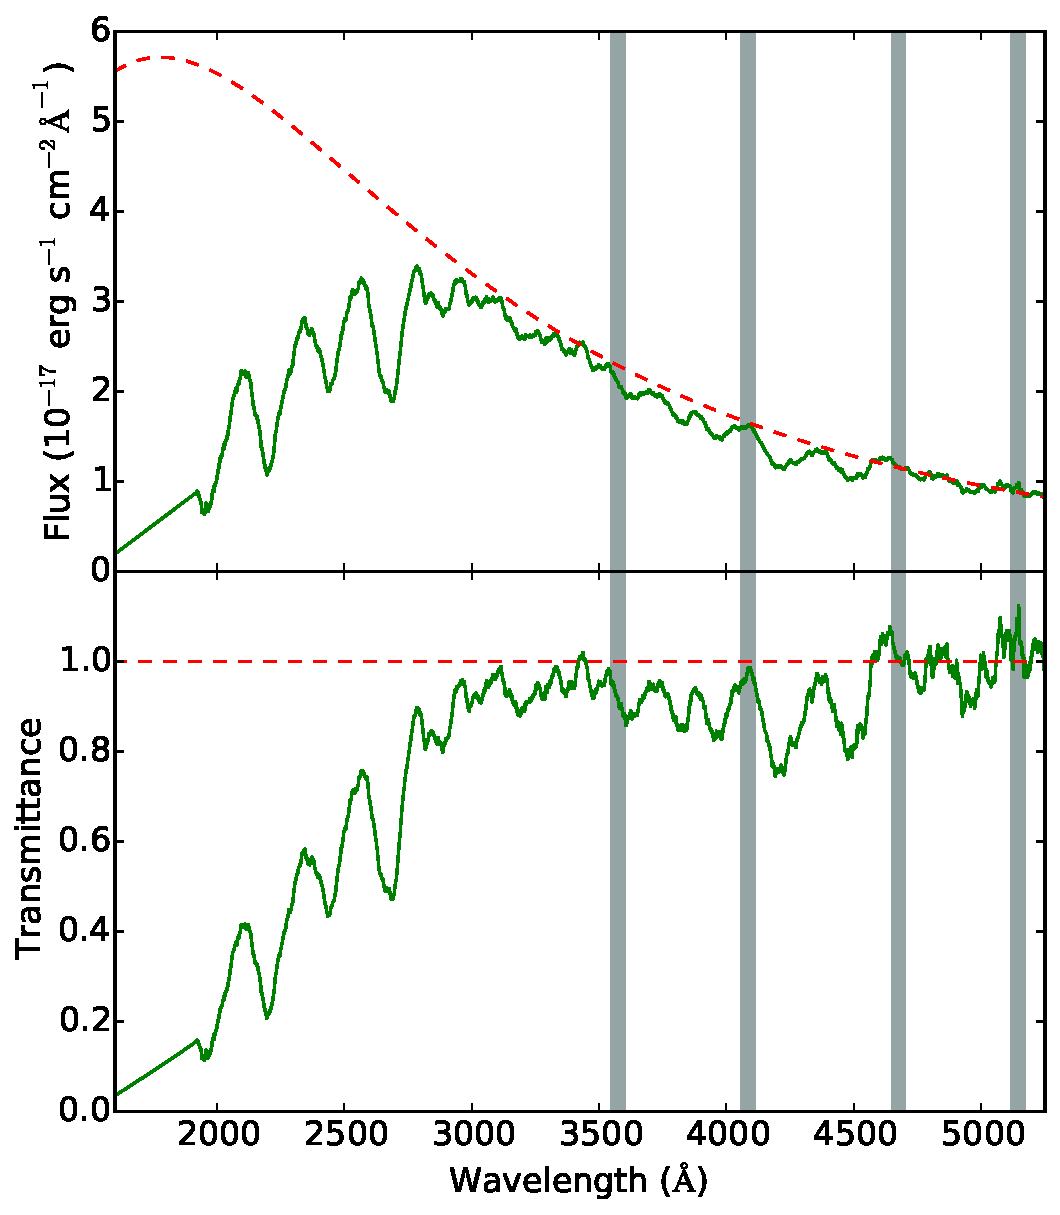
\includegraphics[width=\textwidth]{Figures/Chapter4/specTemplate}
\caption{iPTF13ajg is fitted with the Planck function. The spectrum of iPTF13ajg (green) can shows a good agreement with the blackbody (red) at $\lambda>3000\AA$. At lower wavelengths a strong deviation from the model is observed, highlighting the need for a correction to the model. The ratio between the observed spectrum and the continuum give a measure of the absorption strength as a function of wavelength and can be used in modelling the SLSN SED.}
\label{fig:specTemplate}
\end{figure}

\subsection{Modelling the SED evolution}
The ability to describe the SEDs of SLSNe as blackbodies greatly simplies the
modelling of its evoution. A model is only required to provide the thermal and radial evolution of the photoshere, therefore removing the need for complex modelling such as radiative transfer or hydrodynamic simulations.

\subsubsection{Fireball model}
Perhaps the simplest approach to modelling the SED evolution is to assume that the SN, with an initial radius R$_{0}$ and initial temperature T$_{0}$ expands at a constant rate while cooling down also at a current rate as seen in \eref{eq:Howell}
\begin{align}
\label{eq:Howell}
R(t) &= R_0 + \dot{R}t &&\\
T(t) &= T_0 - \dot{T}t &&
\end{align}
\noindent While this model is not physical motivated, \citet{Howell2013} showed that it provides a good, first-order approximation to the light-curves of SLSNe. Due to its simplicity, the model appeared as an attractive prospect for the modelling of SLSN SEDs. However, our testing showed that while it produces a good fit to a SLSN around the maximum light (<+30days) it is not able to capture the slow evolution in the tale of the light curve as seen in \fref{fig:BB_Mag} making in infavarable in comparison with the more complex magnetar model.

\begin{figure}
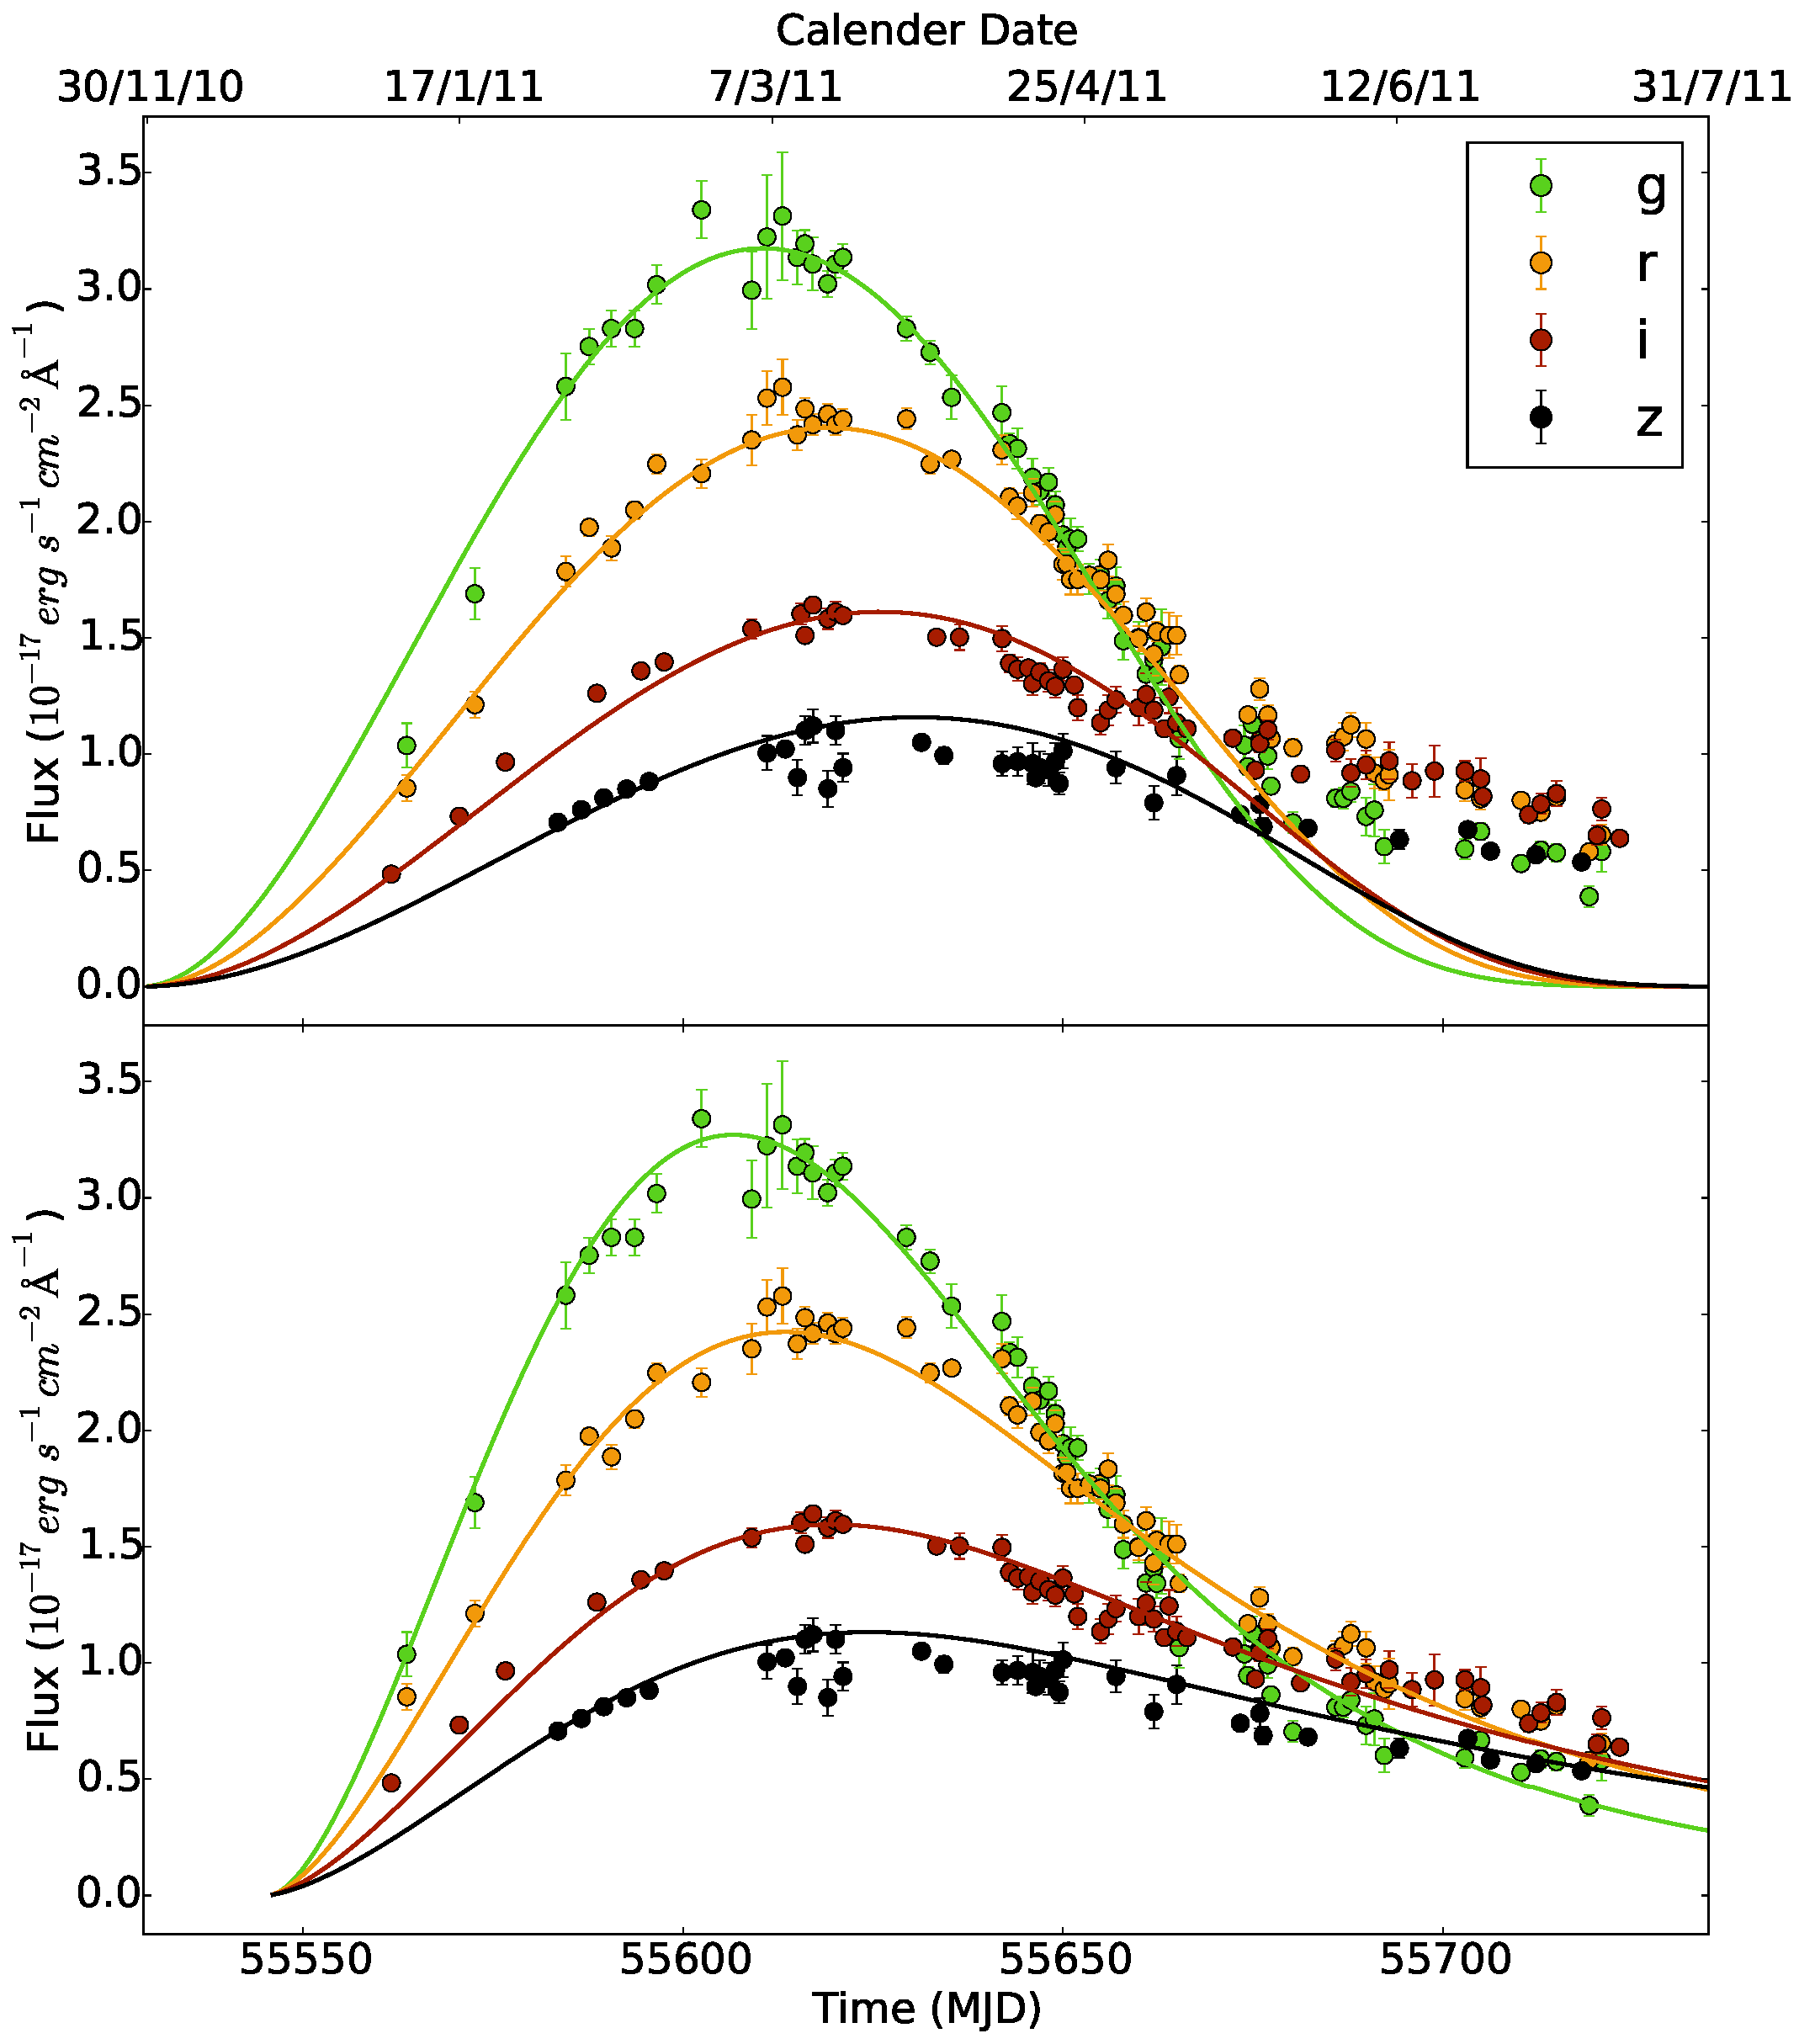
\includegraphics[width=\textwidth]{Figures/Chapter4/BB_Mag_comp}
\caption{The SLSN PS1-11ap $griz$ light curve \citep{2014MNRAS.437..656M} compared to two models describing its photometric evolution. In the upper panel, the model is a simple expanding and cooling blackbody fitted to data around maximum light only, and in the lower panel the model is our `absorbed' magnetar model fitted to the entire light curve. In the case of the magnetar model, the spectrum of SNLS-06D4eu \citep{2013ApJ...779...98H} has been used as an absorption template in the modelling of the SED \sref[see]{sec:KCorrection}). Note that while both models can produce reasonable fits around the peak of the light cuve, the black body model is not able to reproduce the characteristic late-time behaviour of SLSNe. Light curve phases are measured with respect to peak brightness in the rest-frame \textit{u}-band as predicted by our magnetar model fit.}
\label{fig:BB_Mag}
\end{figure}

\subsubsection{Magnetar model}
\label{sec:Magnetar}
To fully capture the evolution of the SED with time we must employ a model for an engine that provides the late time energy deposition needed to explain the photospheric velocity and temperature observed in SLSNe. While still a matter of active debate in literature, in recent years the birth and spin-down of a magnetar model has appeared as the strongest candidate to explain these extremely luminous events \citep{2013ApJ...770..128I,2013Natur.502..346N}. In this model, SLSNe begin as CCSN with a magnetar, a rapidly rotating, highly magnetised neutron star, born at its core. As the magnetar spins down due to the interactions with its environment, it dissipates its energy in the form of high energy radiation that is then captured by the expanding ejecta and thermalised to produce the observed blackbody SED \citep{2010ApJ...717..245K,2010ApJ...719L.204W,2012MNRAS.426L..76D}.

I follow the method from \citet{2013ApJ...770..128I}, based on the Arnett law for the energy diffusion through SN ejecta \citep{Arnett1982}, and the energy radiated by the central engine from \citet{Bildsten2013,Wosley2012}. In order to model the bolometric luminosity, $L$, of a SLSN as a function of time, $t$, we use equation \ref{Eq:MagnetarLum}:
\begin{equation}
L(t) = 4.9\times 10^{46}\,e^{ -(t / \tau_\mathrm{m})^2 }\delta(t) \int_{0}^{t} \frac{2t'}{\tau_\mathrm{m}^2}\,e^{(t'/\tau_\mathrm{m})^2}\,\frac{B_{14}^{2}\,P_{\mathrm{ms}}^{-4}}{\left(1+t'/\tau_\mathrm{p}\right)^2} dt',
\label{Eq:MagnetarLum}
\end{equation}
\begin{equation}
\label{Eq:SDPeriod}
\tau_{p} = 4.7B_{14}^{-2}P_{ms}^{2}days
\end{equation}
\noindent where $\tau_\mathrm{m}$ is the diffusion timescale, $B_{14}$ is the neutron star magnetic field in units of $10^{14}$\,G, $P_{\mathrm{ms}}$ is the magnetar spin period in ms, $\delta(t)$ is the deposition function or trapping coefficient, and $\tau_\mathrm{p}$ is the magnetar spin-down timescale, is defined in \eref{Eq:SDPeriod}, inferred from $B_{14}$ and $P_{\mathrm{ms}}$.

Physically $\tau_M$ is proportional to the ejecta mass($M_{ej}$) which is sometimes chosen as the fit parameter instead. The two parameters can be interconvert using equation \ref{Eq:Mej}, where $E$ is the explosion energy and $\kappa$ the opacity of ejecta.
\begin{equation}
\label{Eq:Mej}
M_{ej} = (\frac{\tau_{M}}{10days})^{4/3}(\frac{\kappa}{0.1cm^2g^{-1}})^{-2/3}(\frac{E_k}{10^{51}erg})^{1/3}M_{\odot}
\end{equation}
\noindent It has been shown \citep{2013ApJ...770..128I,2014ApJ...796...87I,2015MNRAS.452.3869N,2015MNRAS.449.1215P} that the opacity and the explosion energy parameters have only a weak affect the quality of fitting and have therefore been fixed as $\kappa = 0.1cm^2g^{-1}$ and $E = 10^{51}$erg respectively.

The velocity of the ejecta, $v_{core}$ are assumed to be constant and value can be found using the inferred mass of the ejecta, $M_{ej}$ and its kinetic energy, $E_{mag}$ (\eref{Eq:vcore}), which in turn depends on the explosion energy and the energy released by the spin down of the magnetar, shown in \eref{Eq:Emag}:
\begin{align}
\label{Eq:Emag}
E_{mag} = 4.9\times10^{46} B^2 P^{-4} \tau_{P}  \text{ erg} \\
E_k = 10^{51} + 0.5 \times E_{mag} \text{ erg}\\
\label{Eq:vcore}
v_{core} =  \sqrt{\frac{10 E_{k}}{3 M_{ej}}} \text{ cm s}^{-1}
\end{align}

\paragraph{Trapping coofficient}
The trapping coefficient, $\delta(t)$, is defined as the fraction of the high-energy radiation produced by the central engine that gets trapped, and subsequently reproduced as visible light, by the ejecta. It is often assumed in the literature that the trapping coofficient is time-independent and close to unity, implying the full trapping of radiated by the supernova ejecta \citep{2013ApJ...770..128I,2015MNRAS.449.1215P,2015MNRAS.452.3869N}. In this work I use a correction introduced by \cite{2015ApJ...799..107W} with a time-dependent trapping coefficient:
\begin{equation}
\delta(t) = 1 - \exp\left({-\frac{9\kappa \mathrm{M}_{\mathrm{ej}}^{2}}{40\pi  E_k} t^{-2}} \right),
\label{Eq:Wang}
\end{equation}
\noindent where $\mathrm{M}_{\mathrm{ej}}$ is the ejecta mass, $E_k$ is the explosion energy, and $\kappa$ is the opacity. $\mathrm{M}_{\mathrm{ej}}$ is proportional to $\tau_\mathrm{m}$, $E_k$ and $\kappa$ \citep{2013ApJ...770..128I}. We again fix the explosion energy to be $E_k = 10^{51}$\,erg and the opacity as $\kappa =0.1$\,cm$^2$g$^{-1}$.

Using this time-dependent trapping coefficient improves the late-time fit to the light curve. For a typical SLSN we calculate $\delta \simeq 1$ up to 75 days post explosion. However, as the ejecta opacity to high energy photons decreases with time we find $\delta \simeq 0.8$ at 150 days post explosion, emphasising the importance of this correction in the late time light curves.

\paragraph{Deriving Radius and Temperature}
In its simplest form, the magnetar model only predicts the total radiated energy of the SN and does not make any predictions about the SED of the object. It is therefore most commonly used with bolometric light curves, synthesised from the photometry. \citet{2013ApJ...770..128I}, however, shows that it is possible to predict the photospheric radius of a SN based on this model deriving the following equations:
\begin{equation}
\label{Eq:R19}
R(t) = r_{core}(t) \left(\frac{\alpha - 1}{\tau_{core}(t)}\right)^\frac{1}{1 - \alpha}
\end{equation}
\noindent while the radius of the photosphere exceeds that of the core ejecta, and;
\ref{Eq:R20}.
\begin{equation}
\label{Eq:R20}
R(t) = r_{core}(t) - \frac{1 - \frac{\tau_{core}(t)}{\alpha - 1}}{\kappa \rho_{core}(t)}
\end{equation}
\noindent when the photosphere recedes into the core. $r_{core}(t)$, $\rho_{core}(t)=$ and $\tau_{core}(t)$ are defined as follows:
\begin{align}
r_{core}(t) = v_{core}  t \\
\rho_{core}(t)= \frac{3 M_{ej}}{4  \pi  r_{core}^3(t)}\\
\tau_{core}(t) = \kappa  \rho_{core}(t) v_{core} t
\end{align}

Combining this with the total luminosity and assuming that the object radiates as a uniform, spherical blackbody gives us the photospheric temperature. This can be injected into the Planck law to give an approximation for the SED of a SLSN. This method allows for the magnetar model to be fit directly to the multi-band photometry without the need to produce the pseudo-bolometric light curves. We combine this with the absorption templates to produce a model of the SLSN spectral evolution as a function of time.

\subsection{SLAP}
Upon establishing an approach for modelling SLSNe it was important to encapulate it in a software package capable of performing under a number of situations. In this thesis the magnetar model was used in fitting the light curves of both known SLSNe and a variaty of transients, the majority of which could not be well approximated using this model. We have also used it in simulating SLSN in SNLS as well as producing an artificial training sample for the DES machine learning study of SLSNe.

The code was required to satisfy the following requirements:
\begin{itemize}
  \item Fit the magnetar model to all literature SLSNe and estimate their parameters.
  \item Perform a succesful fit to any light curve and return an output, regardless of whether it is physical.
  \item Move the object to any redshift within the range of SNLS and DES.
  \item Allow for the use of any spectral template.
  \item Allow for extensions and modifications to the magnetar model.
  \item Simulate SLSN light curves given input model parameters.
  \item Plot the data and the model, allowing for model comparisons.
  \item Fit light curves on the time scale of minutes and simulate with subsecond performance.
\end{itemize}

The performance requiremets were based on our need to fit the entire archival sample of transients from SNLS as well as regularly fit the live DES transients with an aim of searching for new SLSN candidates. At an average DES cadance of $\sim$5\,days it was necessary that the fitting is performed at a shorter timescale. Similarly, the studies of the rate of SLSNe \cref{Chapter3} and the ML search for SLSNe \cref{Chapter5} required millions of SLSN light curves to be generated for each iterations of the experiment.

After initially testing the model and the fitting methods in the \textsc{Python} langauge environment, I have developed a package that satisfies all of our requirements: The SLSN Lightcurves Analysis Package (SLAP). Written in a combination of \textsc{C++}, \textsc{Cython} and \textsc{Python}, it was used in every project undertaken as part of this thesis. The use of C++ and a number of optimisation techniques allowed for a very large performance improvement versus a similar \textsc{Python} package. \textsc{SLAP} performs model fitting in $\sim$40\,s for an average SNLS light curve and simulated a SLSN in $\sim$10\,ms. The package was published as part of my study of the rate of SLSNe in SNLS \citep{Prajs2016}.

\subsubsection{Code design and structure}
SLAP was designed as a modular, reusable and extendable package while at the same time heavily focussing on the the run-time performance of the code. I have heavily relied on the concepts of Object Oriented Design and Polymorphism to allow me to implement any model as a an extension to the code. At the core of \textsc{SLAP} I have used the concept of approximating the SED of SLSNe as absorbed black bodied. I have defined a virtual \textsc{Model} class that acts as a base class that defined the method for calculating an SED based on the temperature and radius of a SN photosphere. This class is then inherited by a model that defines the time evolution of the SED. This allowed me to use a number of extensions to the base magnetar model that were implemented as plug-ins.

\subsubsection{Model extensions}
While the base magnetar model is a good fit to the majority of SLSNe light curves, in some cases, such as DES14X3taz, it is impossible to fully model the SN without introducing any further assumptions. In this section I will describe a number of magnetar model extensions which I have introduced in order to improve the quality of our fits. It is important to note that these were never used in the simulation of SLSNe for both the rates of SLSNe in \cref{Chapter3} nor the creation of the DES artificial training sample in \cref{Chapter5} as the base model remains a good fit around the maximum light which, in case of the DES and SNLS seasons, is the region observed by our data. The extensions demonstrate the capabilities \textsc{SLAP} and were used only to broaden our understanding of specific, individual objects.

\paragraph{\citet{Piro2015}}
Upon the discovery of DES14X3taz, the question of the engine powering the pre-cursor bump was an important one to answer. \citet{Smith2016} showed that the peak is well explained by a model wherein the supernova explodes inside of an envelope of an extended dense wind. The shock-breakout which is usually observed as a short, $<$1\,day, flash of high energy radiation gets reprocessed into a longer duration emission of lower energy radiation. This model is highly degenerate in the ejecta mass and explosion energy. However, as these parameters also play part in the modelling of the spin-down of a magnetar, the combination of these two models gave us an unprecedented opportunity to derive these parameters directly from the observed data.

In this version of the model, we intoduce a new free parameter, t$_d$, measuring the delay between the explosion of the SN and the onset of the magnetar spin-down. These have not been previosly considered to occur at different times \citep{Nicolls} as there are currently no models that require a delay between the supernova explosion and the formation of the magnetar [ME: NEED TO CHECK THIS, THERE MIGHT BE A PAPER BY WOOSLEY]. However, I have found through the modelling of DES14X3taz that it is impossible to reconcile the magnetar and extended shock models without the introduction of this parameter. Further evidence for is presented in \cref{par:R0nonzero} where the best fit magnetar model for DES14X3taz is shown to require an extended photosphere, consistent with a t$_d ~\sim$ 17days (assuming a constant explansion velocity), in order to better describe the rise phase of the SN.
[ME: MAKE A PLOT FOR THIS]

\paragraph{R$_0~>$ 0}
\label{par:R0nonzero}
While it is widely believed that the birth and a spin-down of a magnetar the most likely progenitor for SLSN, the exact process through which the high-energy radiation produced by the magnetric breaking is transported into the outer shells of the ejecta is not yet understood. If the injection of energy does precisely coincide with the time of explosion of the progenitor star, the SN could go though a "dark" phase followed by a rapid rebrightening. In several cases, including PS1-11ap and DES14X3taz (where we exclude the pre-peak bump data), the magnetar model does not fit the earliest stages of the light curve correctly.

In order to investigate this delay, I have introduced a non-zero initial radius of the progenitor. While the radius of the progenitor star is never null, it is usually negligible in comparison with the expansion velocity of the ejecta. However, in the case of DES14X3taz and PS1-11ap, I found initial radii consistent with ejecta that underwent an expansion at a constant velocity for 17 and XX days respectively. PS1-11ap has no observations prior to its first detections making it impossible to determine if the object was associated with a pre-peak events. This technique, however, can provide insight into the mechanism behind the magnetar energy injection even in the absence of the earliest and pre-explosion epochs. [ME: MAKE A PLOT FOR THIS TOO]

\paragraph{Nickel decay}
Another intersting questions that we were able to investigate using \textsc{SLAP} is the contribution from the radiactive decay of Ni56 and Co56 as an additional energy source powering the ejecta. I have introduced this to investigate a potential mechanism powering the peculiar, flat evolution of DES13S2cmm. In this model, I add the contribution from the decay of these radioactive elements into the bolumetric luminosity of the SN and do not introduce any other modification to the model. While we find that the radioactive decay alone cannot account for the evolution of DES13S2cmm, this test demonstrated the easy with which we are able to modify our models to test new assumptions. The evolution of DES13S2cmm is further investigated in Angus (in prep).

\subsubsection{Maximum Likelihood methods}
The success of \textsc{SLAP} in fitting SLSNe cannot be attributed only to our work on the models but, perhapse in the largest part, to the optimisations applied to the fitting routines. One of the main goals for \textsc{SLAP} was a full autonomation of the fitting process, without the need to manually fine-tunning any input parameters. This is crucial performing fits on large datasets, containing thousands of objects where only a small fraction are likely to be good matches to the model. Furthermore, we do not wish to intruduce any human biases to the fitting procedure, particuarly in the case of the ML training sample as the techniques used by us are sensitive enough to recover such biases over the true trends in the data.

In the early testing phases of the project we have explored fitting the model using the Maximum Likelihood Estimate (MLE) method. This approach is based on maximising the Likelihood function which, in the frequentist approach, describes the probability of the observed data originating from the underlying model. As the uncertainties on our observations are normally distributed I use the Least Squares (LS) regression analysis which is a special case of MLE. In LS fitting, we minimise the residual, defined as the uncertainty weighted difference between the data and a model, using the $\Chi^{2}$ test as a metric for defining the goodness-of-fit:
\begin{equation}
  \Chi^2 = \sum\limits_i^N \left( \frac{O_i - m_i}{\signa_i} \right)^2
\end{equation}

\paragraph{MPFIT}
The MLE fitting approach was implemented in \textsc{SLAP} using \textsc{MPFIT} [CITE], based on \textsc{Fortran}'s well known package \textsc{LMFIT} [CITE]. \textsc{MPFIT} is an implementation of the Levenberg–Marquardt non-linear LS fitting algorithm. This is a popular and highly optimised example of the class of iterative, gradiant descent algorithms that work by traversing the likelihood function, moving in the direction of lower $\Chi^2$ (i.e. higher likelihood). The algoriths use a gradient (either analytical or numerical) of the likelihood function to inform the direction and size of a jump taken at each iteration. In the Levenberg–Marquardt algorith a damping coefficient is introduced decreasing the number of steps taken by the algorithm before converging on a minimum.

While \textsc{MPFIT} was very promising during our testing, we discovered that the quality of our fits strongly dependant on the choice of the initial parameter guesses. This is a common issue amongst all gradient descent algorithms informed only by the gradient at the measured point. This leads to them finding the local likelihood maximum, nearest to the initial parameter guess instead of the global value. This contradicted one of our strongest demands for the package, as \textsc{SLAP} would require manual modification for the initial parameter guesses, making it impossible to use with a large number of objects.

\subsubsection{Bayesian Inference}
While a number of global optimisation approches have been trialed, including parameter grid searches, we realised that the complexity and degeneracies of the magnetar model require a full Bayesian treatment in order to efficiently global minimum (or Maximum Likelihood) of the model. Bayesian Inference is a technique based on the concepts of Bayesian statistics with the goal of maximising the likelihood function defined as:
[EQUATION]
\noindent where the ... is the prior ... evidence

\paragraph{MCMC}
Markov Chain Monte Carlo is a very popular technique for estimating the posterior distribution. In this method a 'walker' moves though the posterior with a large probability of moving towards a higher likelihood value but a non-zero chance of moving towards a lower likelihood value. This is the most striking difference between the fitting performed using MPFIT and MCMC as it is not possible to sample the whole parameter space even if a local minimum has been found the fitter can still go and explore other parts of the posterior.

The added benefit of the Bayesian approach is that essentially as a by product of the calculation we can calculate the Posterior distributuon which tells us the probability of the model.

While this is a great technique with a huge amount of benefits as outlines before it is still very slow and in fact requires even more model evaluations that then grid-search approach. After testing my own custom implementation of the algorithm I also tested a heavily optimised, multitreated package, \textsc{Emcee} [CITE] which has largely accelerated the fitting but not to an acceptable level.

\paragraph{\textsc{MultiNest}}
A recently developed technique for approximating the posterior distribution that shows a much higher efficiency is Nested Sampling [CITE]. Here, the likelyhood is evalued at a number of positions within the prior and then new points are updated based on the evidence of each point. This provides an almost 1000 fold improvement in the efficience of the Bayesian inference performed as compared to the MCMC approach making the algorithm fast enough for the production version of \textsc{SLAP}

In this thesis, I use a Fortran based implementation of the algorithm, \textsc{MultiNest} [CITE]. This is one of the origal implementations of the algorithm. It is very robust and has previously been used in cosmological stufies making it the perfect package for us. On eof its greatest advantages teh posibility of running \textsc{MultiNest} in multi-modal mode where teh resulting fit produces not only the value of best fit but also all modes (or local minima) in the posterior. The output is compatible with the CosmoMC chains giving us a number of tools that can be used to show the posterior distribution and calculate its statistics.

\subsubsection{pyMagnetar}
In order to simulate the light curves of SLSNe we also used \textsc{SLAP} in almost a reverse mode. As the majorority of pipelines and modern tools use Python it was beneficial to wrap the C++ code as a python package. This is done using Cython. [EXPAND]

\section{Searching for Fast Transients}
text
\subsection{Blackbody per epoch}
text
\subsection{Blackbody and spline interpolation}
text
\subsection{Searching for Bumps of SLSNe}
text
\subsection{Searching for Rapidly Evolving Transients}
text

\section{Modeling CCSN}
text
\subsection{CoCo}
text
\subsection{pyCoCo}
text
\subsection{SNIb/c SED UV Extensions}
text
\subsection{SNII with CoCo}
text

\section{Gaussian Processing}
text
\subsection{Theory}
text
\subsection{Choice of Kernels}
text
\subsection{Interpolating Light Curves}
text
